\documentclass[15pt,a4paper]{article}
\pdfoutput=1

\usepackage{amsmath}
\usepackage{float}
\usepackage{graphicx, subfig}
\usepackage{geometry}
\usepackage{caption}
\usepackage{indentfirst}
\usepackage{times}              % set Times New Romans type
\usepackage{setspace}           % set line to line space 
%\usepackage{authblk}            

\geometry{left=2.5cm,right=2.5cm,top=2.5cm, bottom=2.5cm}

\title{\textbf{LOCld55 Design Document}}

\author{\textbf{Author:} Wei Zhang, Di Guo, Quan Sun}


%\affil{College}
\date{\today}

\begin{document}
\begin{spacing}{1.25}           % set line to line space is 1.25
\maketitle

\thispagestyle{empty}           % first page doesn't page number

\newpage

\tableofcontents                % Create contents

\thispagestyle{empty}           % second page doesn't page number

\newpage

\setcounter{page}{1}

\section{General Description of LOCld55}    % Part One

LOCld55 is a \textbf{single-channel, 14Gbps VCSEL driver} ASIC designed under SMIC 55nm CMOS technology. The design follows the references [1][2].

Figure 1 illustrates the block diagram of LOCld55 that includes a laser driver, I2C control unit, and limited amplifier.

%Figure 1: LOCld55 block diagram
\begin{figure}[H]
    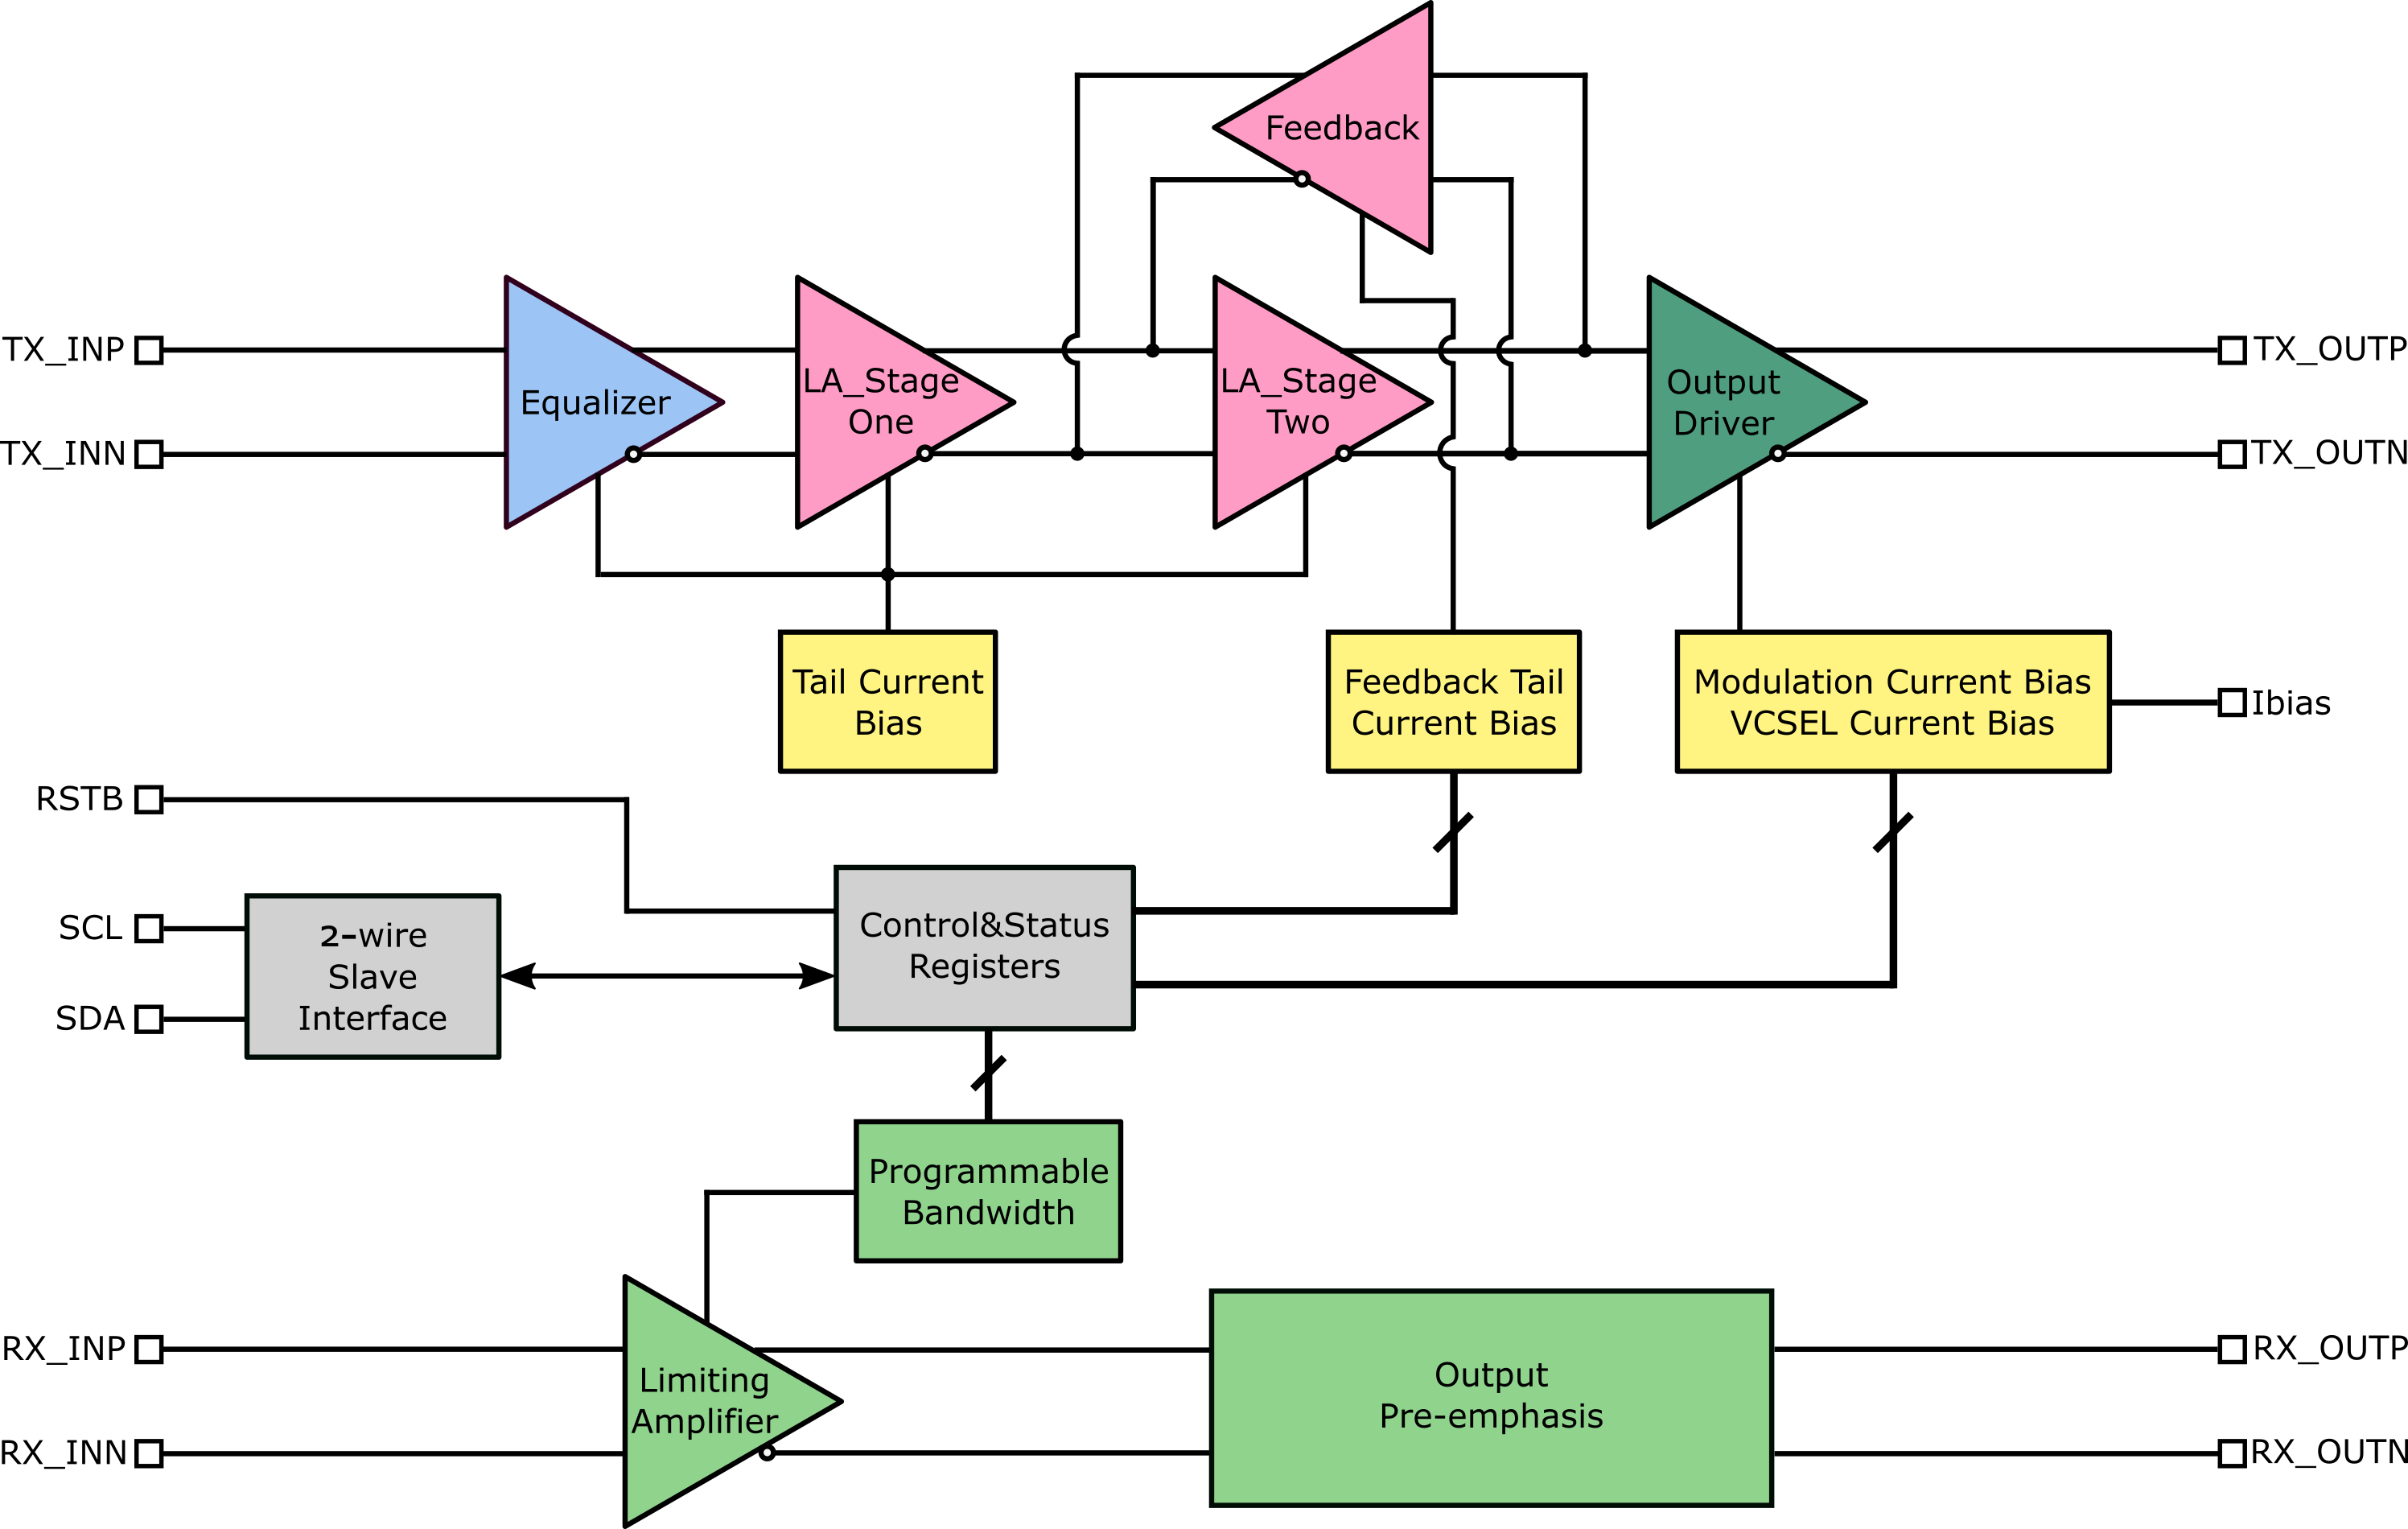
\includegraphics[width=\linewidth]{./Img/locld55.png}
    \caption{LOCld55 block diagram}
%    \lable{Figure 1}
\end{figure}
%Figure 1: LOCld55 block diagram

\section{Pin map of LOCld55}                % Part Two 

\section{Detailed design of LOCld55}        % Part Three
\subsection{Equalizer}

\subsection{Limited Amplifier (LA)}

\subsection{Output Driver (OD)}

\subsection{Equalizer and Limited Amplifier biasing circuit}

\subsection{Modulation bias circuit and Current bias circuit}

\subsection{I2C}

\section{LOCld55 simulation results}        % Part Four

\section{References}                        % Part Five

\end{spacing}
\end{document}
